\documentclass[onecolumn, draftclsnofoot,10pt, compsoc]{IEEEtran}
\usepackage{graphicx}
\usepackage{url}
\usepackage{setspace}
\usepackage{times}
\usepackage{enumitem}
\usepackage{titletoc}
\usepackage{float}
\usepackage{caption}
%\usepackage[export]{adjustbox}
%\usepackage[notocbib]{apacite}
\usepackage{geometry}
\geometry{textheight=9.5in, textwidth=7in}

% 1. Fill in these details
\def \CapstoneTeamName{		Beached Marine Critters Project Team}
\def \CapstoneTeamNumber{		64}
\def \GroupMemberOne{			Alea Weeks}
\def \GroupMemberTwo{			Amar Raad}
\def \GroupMemberThree{			Daniel Domme}
\def \GroupMemberFour{			Justin Disalvo}
\def \GroupMemberFive{			Zachary Tusing}
\def \CapstoneProjectName{		Develop a visual model for sea turtle beach stranding Events}
\def \CapstoneSponsorCompany{	Oregon State University Hatfield Marine Science Center; Oregon Sea Grant}
\def \CapstoneSponsorPerson{		Dr. William Hanshumaker}

% 2. Uncomment the appropriate line below so that the document type works
\def \DocType{		%Problem Statement
				%Requirements Document
				%Technology Review
				Design Document
				%Progress Report
				}
			
\newcommand{\NameSigPair}[1]{\par
\makebox[2.75in][r]{#1} \hfil 	\makebox[3.25in]{\makebox[2.25in]{\hrulefill} \hfill		\makebox[.75in]{\hrulefill}}
\par\vspace{-12pt} \textit{\tiny\noindent
\makebox[2.75in]{} \hfil		\makebox[3.25in]{\makebox[2.25in][r]{Signature} \hfill	\makebox[.75in][r]{Date}}}}
% 3. If the document is not to be signed, uncomment the RENEWcommand below
\renewcommand{\NameSigPair}[1]{#1}

%%%%%%%%%%%%%%%%%%%%%%%%%%%%%%%%%%%%%%%
\begin{document}
\begin{titlepage}
    \pagenumbering{gobble}
    \begin{singlespace}
     \includegraphics[height=3cm]{coe_v_spot1}
        \hfill 
        % 4. If you have a logo, use this includegraphics command to put it on the coversheet.
        %\includegraphics[height=4cm]{CompanyLogo}   
        \par\vspace{.2in}
        \centering
        \scshape{
            \huge CS Capstone \DocType \par
            {\normalsize\today}\par
            \vspace{.5in}
            \textbf{\Huge\CapstoneProjectName}\par
            %\vfill
            \vspace{1in}
            {\Large Prepared for}\par
            \huge \CapstoneSponsorCompany\par
            \vspace{5pt}
            {\Large\NameSigPair{\CapstoneSponsorPerson}\par}
            \vspace{.5in}
            {\large Prepared by }\par
            Group\CapstoneTeamNumber\par
            % 5. comment out the line below this one if you do not wish to name your team
            %\CapstoneTeamName\par 
            \vspace{5pt}
            {\Large
                \NameSigPair{\GroupMemberOne}\par
                \NameSigPair{\GroupMemberTwo}\par
                \NameSigPair{\GroupMemberThree}\par
				\NameSigPair{\GroupMemberFour}\par
			\NameSigPair{\GroupMemberFive}\par
            }
            \vspace{20pt}
        }
        \vfill
        \begin{abstract}
        % 6. Fill in your abstract    
        	%This document is written using one sentence per line.
        	%This allows you to have sensible diffs when you use \LaTeX with version control, as well as giving a quick visual test to see if sentences are too short/long.
        	%If you have questions, ``The Not So Short Guide to LaTeX'' is a great resource (\url{https://tobi.oetiker.ch/lshort/lshort.pdf})
		    \noindent To start to better understand how weather and ocean conditions affect where and when animals get stranded, historical statistics will be combined in a map form to facilitate review by researchers. Geographic Information Systems software will be used to accomplish this goal.  This document lays out the design and functional choices for developing a visual model for sea turtle beach strandings.  Various mock-ups and figures are used to help facilitate understanding.
        \end{abstract}     
    \end{singlespace}
\end{titlepage}
\newpage
\pagenumbering{arabic}
\tableofcontents
% 7. uncomment this (if applicable). Consider adding a page break.
\listoffigures
%\listoftables
\clearpage
\begin{singlespace}
\section{Overview}
    This section provides the basic knowledge required to understand the project.
        
    \subsection{Scope}
    The software outlined in this document is meant to act as a tool to develop a geographic information system (GIS) that will aid in the understanding of why and how sea turtles get stranded. The goal is to develop a user friendly interface where many people of different skills and backgrounds can use the software.
    
    \subsection{Purpose}
    The purpose of this Design Document is to provide an overview of how the group will implement the program. Our goal is to develop a software that will give a visual representation of sea turtle stranding events and the oceanographic conditions that precede these events.
    
    \subsection{Intended Audience}
    The intended audience is our client, William Hanshumaker, and those who will work on the development of the software. This document is intended to be a reference and an overview of how the project will be implemented for any team who wants to create it.
    
    \subsection{Conformance}
    This document conforms to the requirements specified by the client, Dr. William Hanshumaker.
\pagebreak
\section{Definitions}
    This section will provide definitions for all relevant keywords and phrases. \newline \newline
    \textbf{Stranding} - When a sea animal is removed from the water and is unable to reach the water again. This often causes death. \newline \newline
    \textbf{Data Table} - Where data on sea creatures or weather conditions is stored. \newline \newline
    \textbf{Species} - A specific type of animal. \newline \newline
    \textbf{Animal Outcome} - If the animal was found deceased or if it was rehabilitated or assisted into the water. \newline \newline
    \textbf{Map Filters} - Overlays of the map that will allow the user to see a visual representation of the data. \newline \newline
    \textbf{Data Table Filters} - These will allow the user to filter through the data they have available to them.
    \textbf{Component} - A subsection of the program that allows a user to achieve certain design goals. \newline \newline
    \textbf{Visual Model} - A visual representation of data. \newline \newline
    \textbf{GUI} - A graphical user interface. This is the visual representation of the program. This visual representation allows the user to interact with it. \newline \newline
    \textbf{User Interface (UI)} - A user interface is how a user interacts with the program. This is often referenced in correlation with a GUI. This can stand in for a reference of text based or graphical user interface. \newline \newline
    \textbf{Work Space} - The central piece of the user interface. This is where the user will interact with the user interface. The majority of information should be available in this portion. \newline \newline
    \textbf{Input} - A data sheet that fits the specific requirements to provide data to the program.\newline \newline
     \textbf{Geographic Information System (GIS)} - A program designed to process and represent multiple forms of data and layer them over maps [1]. \newline \newline
    \textbf{Olive Ridley Sea Turtle} - A species of sea turtle that is mainly found in warm climates. This species is the primary focus for this project because it gets stranded on Oregon shores [2]. \newline \newline
    \textbf{NOAA} - An abbreviation for Nation Oceanic and Atmospheric Administration. This administration provides scientific data about weather and sea conditions [3]. \newline \newline
    \textbf{NANOOS} - An abbreviation for Northwest Association of Networked Ocean Observation Systems.  This association monitors and studies sea levels and sea life through data collection and visualizations [4]. \newline \newline
    \textbf{Visual Model} - A visual representation of data. Within this project this will provide the user with two separate modeled data. The first is visual representation of the animals location. The second is a visual representation of sea and weather conditions. \newline \newline
   
    
    
\pagebreak  

\section{Conceptual Model for Software Design Descriptions}
This section will include an overview of the software design for the visual model for sea turtle strandings project. This will include a description and figure of how the system architecture is designed. There will be a description of how the models will interact. A description of software design within the software development life cycle will also be discussed. 
        
    \subsection{Software Design Architecture}
    %Note insert diagram here%
    \begin{figure}[H]
    \fbox{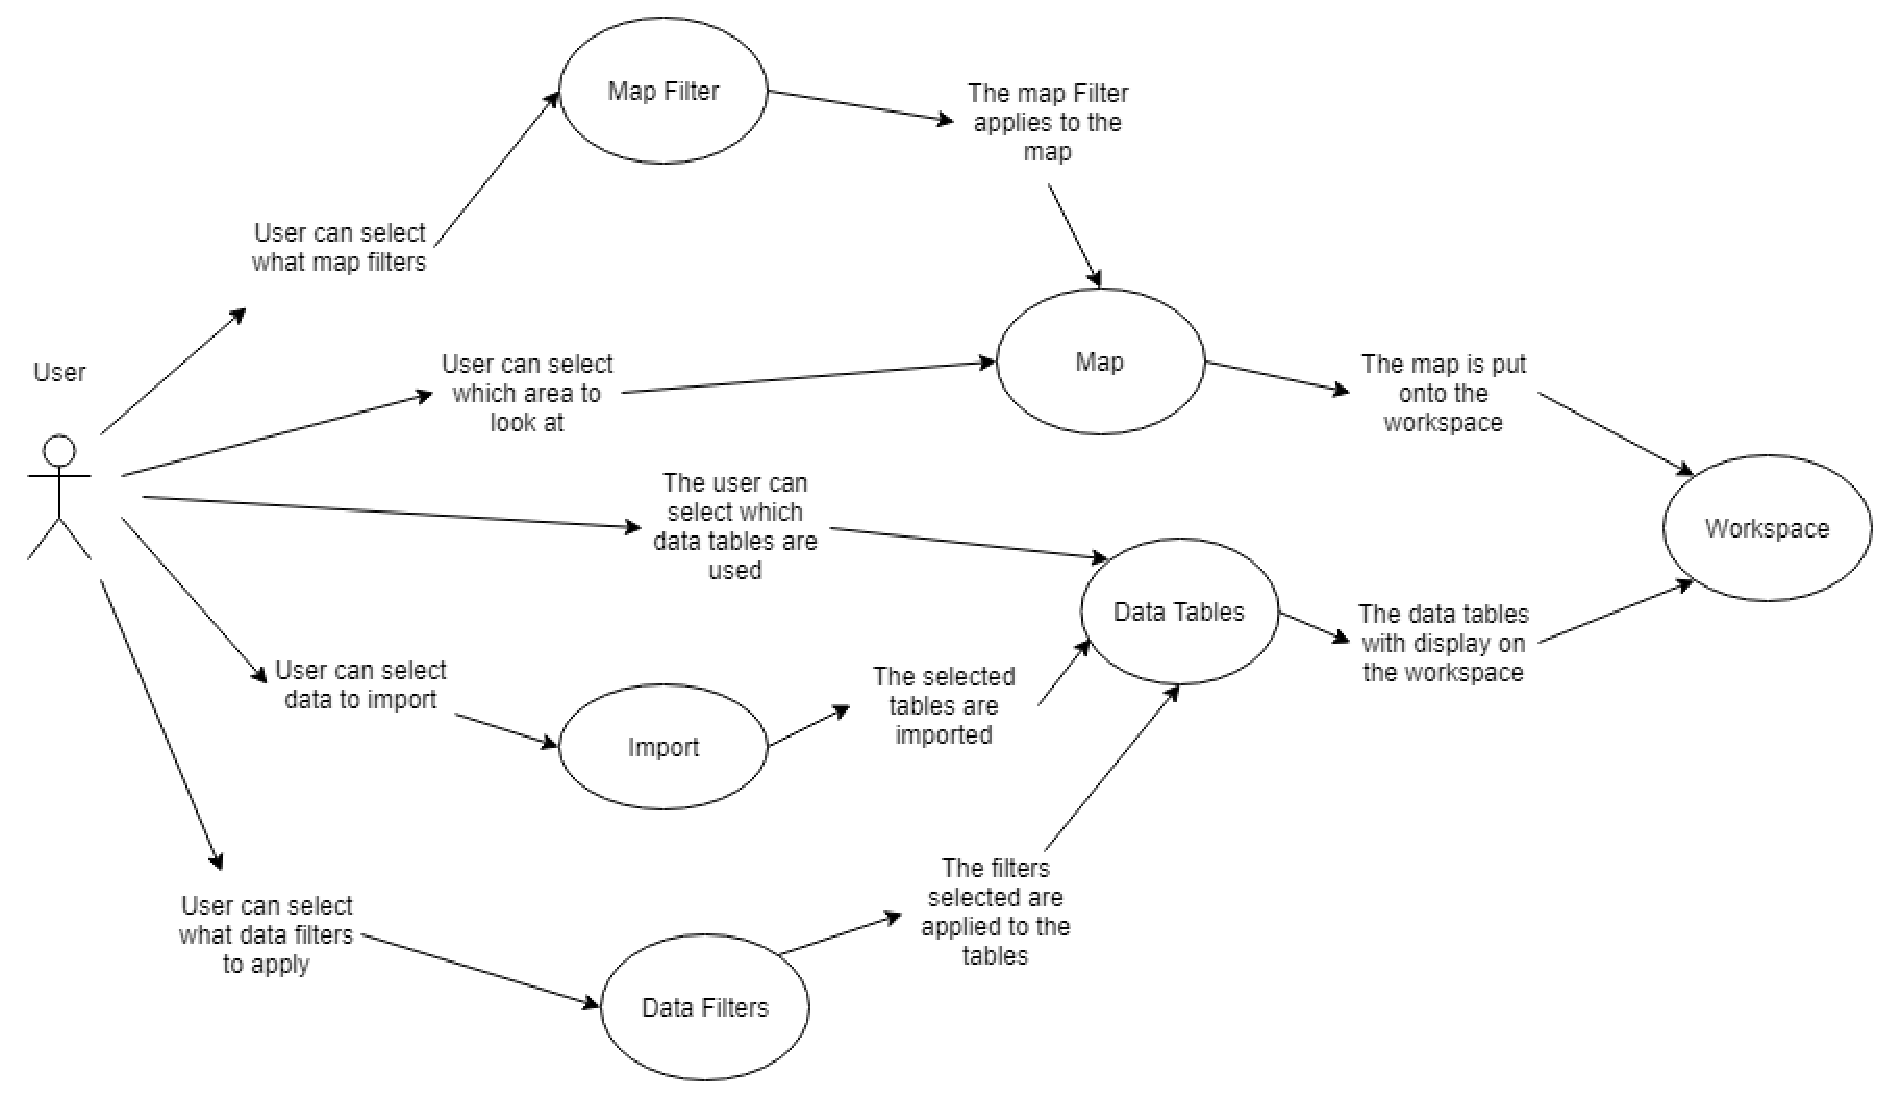
\includegraphics[scale=.6]{updateDiagram.eps}}
    \caption{Software System Architecture}
    \label{fig:SoftwareDesign}
    \end{figure}
        This program will consist of multiple windows that will work within the work space. This will allow the user to interact with multiple different pieces of data within the work space. The work space will consist of a map, map filters, and data tables. These will all be able to be imported into the program and relevant data will be retrieved from files. The map will be provided within it's own window to provide for simple and clear movement. The map filters will be overlay the map and will have a separate selection window. The selection window will allow the user to select individual filters such as weather, tides, etc. The data tables will feed into the map filters providing the filters with information. They will also have a separate window within the work space providing the user the ability to select the data they wish to incorporate. Finally, the data tables will have a filter for a better viewing experience. The user will be able to select which data they wish to incorporate. These windows will all be locked within a larger user interface. 
\pagebreak
    \subsection{Software Design Descriptions within the Life Cycle}
    This program is intended for a Windows operating system. The design choices of this program will allow for the user to add data sets and new information to the program for as long as the user keeps the data formatted in the same manner. This means that the only constraint for the lifespan of this program will be how long the software holds within windows standards. The only foreseeable reason for a standard change would be the move to 128 bit registers (Difference between 32 and 64 bit windows), if this happened it would be highly unlikely the new processors wouldn't be backwards compatible. Therefore, the lifespan of this program is the foreseeable future.
 \pagebreak  
\section{Design Stakeholders and Their Concerns}
    The stakeholders for the development of a visual model for sea turtle beach strandings are the client, William Hanshumaker, those who will use this software in the future, and the team working on the project.  The project team as of 3 December 2018 consists of Alea Weeks, Amar Raad, Daniel Domme, Justin Disalvo, and Zachary Tusing.
    
%NOTE: see IEEE Xplore Full-Text PDF (found on canvas) -> Table 1 -- Summary of design viewpoints (page 13) for more information on Design Viewpoints
\subsection{Design Viewpoints}
    This section describes some of the viewpoints that are applicable to developing a visual model for sea turtle beached stranding. These viewpoints are context, composition, logical, dependency, information, patters, interface, structure, interaction, state dynamics, algorithm, and resource.
    
    \subsubsection{Context Viewpoint}
    When creating the software, it is important to satisfy the stakeholder's requirements. The GUI needs to be simple enough where many people with different levels of computer knowledge will be able to use it and is still able to produce the required output. The users should not be required to have knowledge of databases and how they work.
    
    \subsubsection{Logical Viewpoint}
    The program will use preexisting database files consisting of archival data of stranded sea animals provided by the user.  These files will need to be present on the user's computer, and it will need to be imported in the software.    The inputted data need to include: the species of animal (in this case, sea turtle), date of spotting, location of animal stranding, and condition of animal found.  
    
    \subsubsection{Dependency Viewpoint}
    The state/condition of the weather and ocean's tides are dependant upon the time/day of the reported stranding. Based on when a sea turtle is reported stranded then allows for checking what the corresponding weather and ocean conditions were at that time.
    
    \subsubsection{Information Viewpoint}
    Information regarding the location and time/day (or rough estimate) of a sea turtle's reported stranding will be present. This information will be passed back and stored in the database.
    
    \subsubsection{Interface Viewpoint}
    Users will require an interface that will translate the inputted database into a GIS map that will display the user's data in relation to the location that the animal was found. The user will be able to select different data overlays that will display on top of the original map and data when selected or deselected. These layers include wind direction and velocity, sea surface temperatures, and sea currents.
    
    \subsubsection{Structure Viewpoint}
    Data and design subjects will be organized and sorted in relation to time, chronologically. Following the progression of date and time will show corresponding statistics of the ocean \& weather conditions along with amount of strandings reported.
    
\pagebreak
\section{Component Design}%Daniel begin
    This section will cover component features of the Visual Model for Sea Turtle Beach Strandings software.  Each component is broken down into explaining the user view of the graphical user interface, the structural element in the software, and the reasoning behind the design choices.
    \subsection{Work Space}
        \subsubsection{GUI Element}
        The work space is the GUI environment that the user views and manipulates data.  This is the basis of implementation for other features.  The work space allows for the importation and analysis of animal stranding reports in tandem with oceanic and weather conditions.

            \begin{figure}[H]
            \fbox{\includegraphics[width=\textwidth]{nodata.eps}}
            \caption{Work Space Environment}
            \label{fig:Mockup}
            \end{figure}
            
        \subsubsection{Structural Element}
        The organization of the work space should be set up to allow most of the information to be viewed at once, and it should be easy to understand.  The background should not draw attention, and the colors should be chosen to include people with color blindness.  It should also aid in the display of information.  The work space should include as many common functionalities as possible to allow ease of use.  This means that menu trees will follow standard layouts and content.  Language of functions will also follow widespread norms.
        \subsubsection{Design Rationale}
        By using standard designs and layout of the graphical user interface, the user will start their experience with a familiar base to start to learn how to use the software.  This should foster a positive work environment.
        
    \subsection{Import}
        \subsubsection{GUI Element}
        The import button will allow the user to import data sets into the map and data table for inclusion in analysis. This button is situated at the top of the work space in line with the other menu buttons.
        \subsubsection{Structural Element}
        When selected by the user, a window menu will pop up to prompt the user to select a file to import into the program.  The user will be able to browse files on their computer to find the specified file.  The supported data files will be Microsoft Excel file formats.  At the very least, the data must include distinct reports with animal species, animal find date, and animal find location.  The animal find location may be a general area such as city name or beach name, but map coordinates are preferred.
        \subsubsection{Design Rationale}
        Providing the single-use button for the importation of data files helps to minimize searching done by the user.  It plainly lays out the function in a convenient space. Enforcing data file format requirements allows for a more reliable software experience and performance.  The software can be more focused and less time can be used in supporting more variations of data types.  Using a standard category names means that the data can be more thoroughly examined. 
    \subsection{Map}
        \subsubsection{GUI Element}
        The map element of the software is the primary function of the software application.  It takes up the most amount of screen space, and it is centrally located in the work space below the menu buttons.
        \subsubsection{Structural Element}
        The map is included in our software download for the user.  This map will come from the ArcGIS software.  The map will utilize common standard user manipulation techniques such as using the mouse to interact.  The user will be able to zoom in and out by using the scroll wheel, and they will be able to drag the map to change the focus of the viewpoint.  The user will also be able to select data points on the map and zoom in on that point.  The map will have overlays for sea and weather conditions that will provide more data to the user. There are buttons on the map that allow a user to manipulate the view as an alternate way to scroll and zoom.
        \subsubsection{Design Rationale}
        Prominently locating the map and giving the most screen space will make viewing large areas of the map with scattered data points with overlays easier.  The user will be able to widen the scope of regional weather and sea conditions and look for varying conditions.  Having common user interaction methods helps to create a natural and intuitive environment to accomplish analyzing data and minimize time becoming familiar with the software.
        \subsection{Map Overlays}
            \subsubsection{GUI Element}
            The map overlays check box filters will allow the user to apply data filters on top of the base map.  The overlays are surface currents, surface temperature, and wind speed and direction.
            \subsubsection{Structural Element}
            The user can choose to check as many of the map overlays that they want at a given time.  These overlays will apply over the base map.  The base map will still be visible, and the overlays will be distinct to allow for easy interpretation of data and interactions.
            \subsubsection{Design Rationale}
            The choice of using check boxes to select and deselect overlays makes clear that the options are optional and can be chosen in any order.  They allow for rapid transition of data to be displayed in tandem to animal stranding reports.  The user will be able to view all data at the same time in an easily understandable way without having to rapidly change between views to analyze data.
    \subsection{Turtle Selection}
            \subsubsection{GUI Element}
            The turtle selection check box filters allow for the user to select which species of turtles are displayed on the map.
            \subsubsection{Structural Element}
            The user will be able to select as many species from the filter box that they desire.  The boxes that are checked are the species that will be displayed.
            \subsubsection{Design Rationale}
            Giving the ability to select certain species to display on the map allows the user to focus on turtles that might be pertinent to research.  In addition, different species of turtles have different properties and native environments.  Choosing to not include some species can help to eliminate correlations from being skewed, and correlations can be drawn for each species.
    \subsection{Data Table}
        \subsubsection{GUI Element}
        The data table to displays all data points that have been imported by the user.  The table is intended to aid the user to be able to understand what data is included and select individual data points.  The data table element is positioned less prominently than the map.  It will be on the side of the map to be able to view it at the same time as the map.  The list of data will be scrollable with a scroll bar to indicate scroll position.
        \subsubsection{Structural Element}
        The data table will be a list of all imported data that the user has provided.  The data table will be held in memory by the program and sorted as needed.  The list will be able to be scrolled through on both the horizontal and vertical axes.  If the user wishes to see more details of a data element, they can scroll left or right to view the information.  Selecting or mousing over will highlight the element in the table and on the map.  The elements will be number and distinct to aid in the viewing and understanding of the data.
        \subsubsection{Design Rationale}%Daniel end
        The position of the data table next to the map will help the user to be able to find information about a particular point easily with more detail.  It also means that the user does not have to change views and have to memorize information between elements.  The table allows for quick glances and access of elements for the user's convenience.  Being able to scroll through the data allows the user to focus on particular elements and to not get overwhelmed with information.
    \subsection{Map Filters}
        \subsubsection{GUI Element}
        The map filters will be positioned above the map. It will be less predominant than the map but still easily in view. There will be various map filters to select from
        \subsubsection{Structural Element}
        The map filters will be displayed in a box above the main display map. The filters will consist of various data that can either be overlayed onto the map or can be used to limit/expand data shown on the map. Options for map filters will include the following. There will be a date selection box where a user can enter in a specific date they would like to see data for, this would limit the data shown on the map to only data from only the user specified date. Similarly, there will be a date range the user can specify, this will only show data from the user specified date range. Finally, the user can select overlays to be applied to the map. Under overlay selection, the options surface currents, surface temperature, and wind speed will be listed with checkboxes next to them. The user can check these and have the map overlayed with the data they've selected.
        \subsubsection{Design Rationale}
        The position of the map filters above the map puts them in an easily visible spot. The map filters are accompanied with intuitive user actions such as checking checkboxes to update the map. Since the map filters are positioned above the map, it makes it so the user can easily see what filters are applied and how they affect the data shown on the map.
    \subsection{Data Table Filtering}
        \subsubsection{GUI Element}
        The position of the data table Filtering options will be to the top right of the map and above the data table element. It will be a list where the user can select one option.
        \subsubsection{Structural Element}
        The data table Filtering options will be in a box located to the upper right of the map. It will contain options for Filtering the data such as by species, date, location, animal outcome, and animal age. Next to each option will be a radio button that allows the user to select one option from the list. After the user has selected an option, the data table will update and be sorted by the user specified option. 
        \subsubsection{Design Rationale}
        The position of the data table Filtering options above the data table is appropriate since they will apply directly the the data table. Having the elements next to each other makes it so the user does not need to search around for either one. 
\pagebreak
\section{User Interface}
    This section will contain an overview of the user interface (UI) for the Visual Model for Sea Turtle Beach Strandings software. Included is a description of the UI's various components and functionality. User interface mock ups that demonstrate the UI are also included in this section. 
        
    \subsection{User Interface Overview}
    The graphical user interface of the Visual Model for Sea Turtle Beach Strandings application intended to be a positive and intuitive experience for any user who is familiar with computers.  The layout of the menu functions fosters quick and clear actions in a familiar manner. The application is designed in a way that does not require much familiarization and learning to use.  In addition, the cognitive load of the user is minimized by displaying information in one view.  The user is not required to memorize information between screens, and data can be viewed and manipulated with few mouse movements and clicks.  Interfacing with the map is in a universally standard format.  This allows the user to manipulate it using only the mouse with clicks, drags, and scrolls.  The displayed data can be changed by checking and unchecking simple boxes, and the data can be sorted using a selector.
    
    \subsection{Screen Images}
        \begin{figure}[H]
        \fbox{\includegraphics[width=\textwidth]{nodata.eps}}
        \caption{Work Space Environment Upon Start up with No Data}
        \label{fig:Mockup1}
        \end{figure}
        
        \begin{figure}[H]
        \fbox{\includegraphics[width=\textwidth]{browse.eps}}
        \caption{Import Button Selection Menu}
        \label{fig:Mockup2}
        \end{figure}
        
        \begin{figure}[H]
        \fbox{\includegraphics[width=\textwidth]{fullMockup.eps}}
        \caption{Work Space with Data Imported and Displayed}
        \label{fig:Mockup3}
        \end{figure}
        
        \begin{figure}[H]
        \fbox{\includegraphics[width=\textwidth]{selectData.eps}}
        \caption{Data Element Selected}
        \label{fig:Mockup4}
        \end{figure}
        
        \begin{figure}[H]
        \fbox{\includegraphics[width=\textwidth]{dataSort.eps}}
        \caption{Data Elements Sorted By Location}
        \label{fig:Mockup5}
        \end{figure}
        
        \begin{figure}[H]
        \fbox{\includegraphics[width=\textwidth]{selectDataOverlays.eps}}
        \caption[Work Space with Data and Overlays Selected]{Work Space with Data and Overlays Selected\cite{windyMap}}
        \label{fig:Mockup6}
        \end{figure}

\renewcommand\refname{Bibliography}

% bibliography
\pagebreak
\nocite{*}%if nothing is referenced it will still show up in refs
\bibliographystyle{IEEEtran}
\bibliography{refs}

\end{singlespace}
\end{document}